\documentclass[11pt]{article}
\usepackage[italian]{babel}
\usepackage{geometry}
\usepackage{graphicx} 
\geometry{a4paper} 
\usepackage{listings} % necessario per inclusione codice sorgente
\usepackage{color} % syntax highlighting
\usepackage{url}
% qualsiasi altro package necessario può essere aggiunto qui ...

% definizione dei colori  
\definecolor{dkgreen}{rgb}{0,0.6,0}
\definecolor{gray}{rgb}{0.5,0.5,0.5}
\definecolor{mauve}{rgb}{0.58,0,0.82}

\pdfinfo{
   /Author (Andrei Ciulpan)
   /Title  (Specifica del Progetto di Laboratorio - Architetture I - Turno A)
}
\title{Specifica del Progetto di Laboratorio \\ Architettura degli Elaboratori I}
\author{Andrei Ciulpan\\ Matricola: 872394 - Turno: A\\ \url{andrei.ciulpan@studenti.unimi.it}}
\date{}

\begin{document}
\maketitle

\section{Guitar Hero in Logisim}

Il progetto consiste nella realizazzione di un circuito che simula il gioco, ormai famoso,
Guitar Hero. Il gioco avrà come board di gioco una matrice LED 8x8 (come in Figura
1) dove cadranno dei ”tiles” in maniera casuale e l’utente potrà interagire con la
board attraverso 4 bottoni. L’utente dovrà schiacciare il bottone al momento opportuno
(ovvero quando i ”tiles” arrivano nella prima riga della matrice LED) per guadagnare
punti (il punteggio degli HIT verrà visualizzato su due hex digit display). Se l’utente
non schiaccerà il bottone al momento opportuno allora verrà incrementato il contatore
dei MISS (questo verrà visualizzato su un hex digit display). Il gioco terminerà dopo
aver guadagnato 20 punti oppure dopo aver sbagliato 9 volte. Il gioco terminerà con la
visualizzazione di un messaggio su una matrice LED ("YOU WON" oppure "YOU LOST").
Ci saranno presenti pulsanti per ON/OFF e RESET.

\begin{figure}[!htpb]
\centering
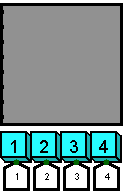
\includegraphics[width=0.3\columnwidth]{immagini/board_di_gioco}
\caption{Screenshot della board di gioco}
\label{fig:fig1}
\end{figure}

\end{document}
